

\clearpage
\tableofcontents

\clearpage
\section{Definition}

In this section, I firstly describe several definitions used in the following contexts.

\subsection{Price Change Patterns}

The Price Change Patterns are categorized into uni-variant price change patterns and bi-variant price change patterns. The motivation for such categorization is to provide a ``lower'' level sense (using uni-variant price change patterns) to facilitate the understanding of difference across bi-variant price change patterns.

\begin{table}[H]
	\caption{Definition: Price Change Patterns}
	\begin{tabular}{lll}
		\hline\hline
		Price Change Patterns &   Symbol    & Definition                          \\ \hline\hline
		1                     & \texttt{D } & Uni-price-change pattern: Decrease  \\
		2                     & \texttt{I } & Uni-price-change pattern: Increase  \\
		3                     & \texttt{N } & Uni-price-change pattern: No Change \\ \hline
		& \texttt{. } & Uni-price-change pattern: Missing   \\ \hline\hline
		4                     & \texttt{DD} & Bi-price-change pattern             \\
		5                     & \texttt{II} & Bi-price-change pattern             \\
		6                     & \texttt{DN} & Bi-price-change pattern             \\
		7                     & \texttt{IN} & Bi-price-change pattern             \\
		8                     & \texttt{DI} & Bi-price-change pattern             \\
		9                     & \texttt{UU} & Bi-price-change pattern             \\ \hline
		& \texttt{D.} & Bi-price-change pattern             \\
		& \texttt{I.} & Bi-price-change pattern             \\
		& \texttt{N.} & Bi-price-change pattern             \\
		& \texttt{..} & Bi-price-change pattern             \\ \hline\hline
	\end{tabular}
\end{table}

There are 4 uni- and hence 10 bi- variant price change patterns, as the order does not matter, i.e., combination. Of the 14 price change patterns, 9 (numbered) are of interest and hence enter the calculation and tabulation in the following.

I use uni-PCP to refer to uni-variant price change pattern, and bi-PCP to bi-variant price change pattern in this report.

\subsection{Group}

The definitions of groups are as follows.

\begin{table}[H]
	\caption{Definition: Groups}
	\begin{tabular}{l|rrrrrrr}
		\hline\hline
		Group & Year & Name & Country & Good & Variety & Variety2 & Variety3 \\ \hline\hline
		gp-1  &  yes &  yes &         &      &         &          &          \\
		gp-2  &  yes &      &         &  yes &         &          &          \\
		gp-3  &  yes &      &         &  yes &     yes &          &          \\
		gp-4  &  yes &  yes &         &  yes &         &          &          \\
		gp-5  &  yes &  yes &         &  yes &     yes &          &          \\ \hline\hline
		gp-A  &      &  yes &     yes &      &         &          &          \\
		gp-B  &      &  yes &         &  yes &         &          &          \\
		gp-C  &  yes &  yes &         &      &         &          &          \\
		gp-D  &  yes &  yes &     yes &      &         &          &          \\
		gp-E  &  yes &  yes &     yes &  yes &         &          &          \\ \hline\hline
		gp-6  &  yes &      &         &      &         &      yes &          \\
		gp-7  &  yes &  yes &         &      &         &      yes &          \\
		gp-8  &  yes &      &         &  yes &         &      yes &          \\
		gp-9  &  yes &  yes &         &  yes &         &      yes &          \\ \hline
		gp-10 &  yes &      &         &      &         &          &      yes \\
		gp-11 &  yes &  yes &         &      &         &          &      yes \\
		gp-12 &  yes &      &         &  yes &         &          &      yes \\
		gp-13 &  yes &  yes &         &  yes &         &          &      yes \\ \hline\hline
		gp-F  &      &  yes &         &      &         &      yes &          \\
		gp-G  &      &  yes &     yes &      &         &      yes &          \\
		gp-H  &      &  yes &         &  yes &         &      yes &          \\
		gp-I  &  yes &  yes &         &      &         &      yes &          \\
		gp-J  &  yes &  yes &     yes &  yes &         &      yes &          \\ \hline
		gp-K  &      &  yes &         &      &         &          &      yes \\
		gp-L  &      &  yes &     yes &      &         &          &      yes \\
		gp-M  &      &  yes &         &  yes &         &          &      yes \\
		gp-N  &  yes &  yes &         &      &         &          &      yes \\
		gp-O  &  yes &  yes &     yes &  yes &         &          &      yes \\ \hline\hline
	\end{tabular}
\end{table}

Groups 1-5 are defined to study the price coordination acorss countries/regions, and therefore, do not include country identification variable; groups a-e are defined to study the price coordination within certain name groups and hence all include name identification variable.

Groups 6-9 and 10-13 are defined similarly to groups 1-5, using new variety variables; groups f-j and k-o are defined similarly to group a-e, also using new variety variables.

\subsection{Price Changes}

The definitions of price changes are as follows.

\begin{table}[H]
	\caption{Definition: Price Changes}
	\begin{tabular}{l|l|rrrrrr}
		\hline\hline
		Price Changes & Variables  & $ (-\infty,-1) $ & $ [-1,0) $ & $ [0,0] $ & $ (0,1] $ & $ (1,\infty) $ & Missing \\ \hline\hline
		pc-1          & pcf        &           $ -1 $ &     $ -1 $ &     $ 0 $ &     $ 1 $ &          $ 1 $ &       . \\
		pc-2          & pc\_pennyf &           $ -1 $ &      $ 0 $ &     $ 0 $ &     $ 0 $ &          $ 1 $ &       . \\
		pc-3          & pc\_unitf  &                . &     $ -1 $ &     $ 0 $ &     $ 1 $ &              . &       . \\
		pc-4          & pc\_allf   &           $ -2 $ &     $ -1 $ &     $ 0 $ &     $ 1 $ &          $ 2 $ &       . \\ \hline\hline
	\end{tabular}
\end{table}

One side-note for price changes are that, the program are set to be compatible with the first three price change definitions, and not with the last price change definition.

%\subsection{Occurrence (OCC) \& Frequency (FRQ); Conditional (CON)}
%
%Throughout the study, three statistics, Occurrence, Frequency and Magnitude, are reported. The following example illustrate how OCC and FRQ  are defined using CON.
%
%Suppose the following group.
%\begin{center}
%	\begin{tabular}{llll}
%		\hline\hline
%		Group & Observation & Indicator & Level \\ \hline
%		1     & 1           & I         & 0.80  \\
%		1     & 2           & I         & 0.06  \\
%		1     & 3           & .         & .     \\
%		1     & 4           & N         & 0.00  \\
%		1     & 5           & N         & 0.00  \\ \hline\hline
%	\end{tabular}
%\end{center}
%Then the OCC is the number of occurrence of each price change patterns, both uni- and bi- variant.
%\begin{center}
%	\begin{tabular}{l|rrrrrrrrr}
%		\hline\hline
%		PCP & D & I & N & DD & II & DN & IN & DI & NN \\ \hline
%		OCC & 0 & 2 & 2 &  0 &  1 &  0 &  4 &  0 &  1 \\ \hline\hline
%	\end{tabular}
%\end{center}
%The CON calculation takes an extra step by replacing the ZERO to NAN; the logic of using conditional definition is as follow.
%\begin{center}
%	\begin{tabular}{l|rrrrrrrrr}
%		\hline\hline
%		PCP &  D & I & N & DD & II & DN & IN & DI & NN \\ \hline
%		OCC & -- & 2 & 2 & -- &  1 & -- &  4 & -- &  1 \\ \hline\hline
%	\end{tabular}
%\end{center}
%The FRQ is calculated as share of the total number of OCC, separating uni- and bi- variant PCPs.
%\begin{center}
%	\begin{tabular}{l|rrrrrrrrr}
%		\hline\hline
%		PCP &  D &    I &    N & DD &   II & DN &   IN & DI &   NN \\ \hline
%		OCC & -- &    2 &    2 & -- &    1 & -- &    4 & -- &    1 \\
%		FRQ & -- & 0.50 & 0.50 & -- & 0.17 & -- & 0.67 & -- & 0.17 \\ \hline\hline
%	\end{tabular}
%\end{center}
%
%\subsection{Magnitude (MAG)}
%
%I report three MAGs. Continue with the previous example.
%
%The MAG of uni-PCP is the average of absolute values of uni-PCP levels.
%\[ \texttt{MAG I} = 0.43 = (|0.80| + |0.06|) /2 \]
%\[ \texttt{MAG N} = 0.00 = (|0.00| + |0.00|) /2 \]
%
%The MAG of bi-PCP is the average of absolute values of bi-PCP level differences.
%\[ \texttt{MAG II} = 0.37 = (|0.80 - 0.06|) /1 \]
%\[ \texttt{MAG IN} = 0.43 = (|0.80 - 0.00| + |0.80 - 0.00| + |0.06 - 0.00| + |0.06 - 0.00|) /4 \]
%\[ \texttt{MAG NN} = 0.00 = (|0.00 - 0.00|) /1 \]
%
%The MAG of uni-PCP in bi-PCP is the average of absolute values of uni-PCP levels used in forming that bi-PCP.
%\[ \texttt{AVG I in II} = 0.43 = (|0.80| + |0.06|) /2 \]
%\[ \texttt{AVG I in IN} = 0.43 = (|0.80| + |0.80| + |0.06| + |0.06|) /4 \]
%\[ \texttt{AVG N in IN} = 0.00 = (|0.00| + |0.00| + |0.00| + |0.00|) /4 \]
%\[ \texttt{AVG N in NN} = 0.00 = (|0.00| + |0.00|) /2 \]
%
%Therefore, the previous example can be extended.
%\begin{center}
%	\begin{tabular}{l|rrrrrrrrr}
%		\hline\hline
%		PCP  &  D &    I &    N & DD &   II & DN &   IN & DI &   NN \\ \hline
%		OCC  & -- &    2 &    2 & -- &    1 & -- &    4 & -- &    1 \\
%		FRQ  & -- & 0.50 & 0.50 & -- & 0.17 & -- & 0.67 & -- & 0.17 \\
%		MAG  & -- & 0.43 & 0.00 & -- & 0.37 & -- & 0.43 & -- & 0.00 \\ \hline
%		AVGD & -- &   -- &   -- & -- &   -- & -- &   -- & -- &   -- \\
%		AVGI & -- & 0.43 &   -- & -- & 0.43 & -- & 0.43 & -- &   -- \\
%		AVGN & -- &   -- & 0.00 & -- &   -- & -- & 0.00 & -- & 0.00 \\ \hline\hline
%	\end{tabular}
%\end{center}

\subsection{At \& Between Percentiles}

In price coordination analyses across the sizes of groups, the AT-percentile tabulates the average using observations exactly at the percentile; for example, the at-60-percentile tabulates the average using observations in $ (59,60] $ percentile range. On the other hand, the BETWEEN-percentile tabulates the average using observations between the percentiles; for example, the between-60-percentile tabulates the average using observations $ (50,60] $ percentile range.

\subsection{Countries \& Regions}

There are seven countries, US, UK, Canada, France, Italy, Germany, and Sweden.

I define three regions first. Region EU contains countries that shares Euro dollars, including France, Italy, and Germany; region NA contains countries in North America, including US, and Canada; region NO includes all the countreis that does NOT share Euro dollars, including US, Canada, UK, and Sweden, i.e., NA, and UK and Sweden.

The two cross-region cases are EUNA and EUNO. EUNA selects one country from EU region and one from NA region; EUNO selects one country from EU region and one from NO region.

\clearpage
\section{Price Coordination}

In this section, the study of price coordination is conducted. As indicated by the tiles of following subsections, the study contains three parts; specifically,
\begin{itemize}
	\item price coordination within name groups,
	\item price coordination within name groups across group sizes, and
	\item price coordination within and across regions.
\end{itemize}
Analyses are done using all the group and price change definitions aforementioned.

\subsection{Price Coordination Within Name Groups}

\paragraph{What Is Tabulated}

In this subsection, I report the summary statistics for study of price coordination within name groups. Throughout this section, the price change definition is PC-1, i.e.,
\begin{itemize}
	\item \texttt{pcf}.
\end{itemize}
I report results for groups D, E, J, and O. The definitions of them are repeated as follows. Note that in previous analyses, the group definition is set as in GP-D.
\begin{itemize}
	\item GP-D: (name,year,country)
	\item GP-E: (name,year,country,good)
	\item GP-J: (name,year,country,good,variety2)
	\item GP-O: (name,year,country,good,variety3)
\end{itemize}
The summary statistics are defined as in previous section. Studying price coordination, one is particularly interested in frequency row-(2) of each panels across bi-variant price change patterns.

\paragraph{What Can Be Said}

See Table \ref{tbl1}. Moving from GP-D to GP-E, i.e., adding good as an additional identification variable for group definition, sees three changes.
\begin{enumerate}
	\item Both frequencies of DD and II increase.
	\item Both frequencies of DN and IN decrease.
	\item The frequencies of DI decrease.
\end{enumerate}
All the three changes suggests, adding additional identification variable strengthen the price coordination within name groups. (This is also supported by comparing GP-A, -B and -C to GP-D and -E.)

Moving from GP-E to GP-J and -O has only marginal effects.
\begin{itemize}
	\item Adding additional identification variables of variety does not increase the price coordination within name groups. (TODO: Review variety2 and variety3 definitions.)
	\item Generally, the price coordination seems to increase substantially from GP-D to GP-E, and to remain at the same level in GP-E, -J and -O.
\end{itemize}

\begin{table}[H]
	\caption{Price Coordination Within Name Groups}\label{tbl1}
	\begin{tabular}{llrrrrrrrrr}
		\hline\hline
		& Stat &     D &     I &     N &    DD &    II &    DN &    IN &    DI &     NN \\ \hline\hline
		GP-D &      &       &       &       &       &       &       &       &       &        \\
		(1)  & OCC  &  6726 & 11591 & 41724 & 17056 & 39007 & 48088 & 77247 & 12996 & 262420 \\
		(2)  & FRQ  & 0.112 & 0.193 & 0.695 & 0.037 & 0.085 & 0.105 & 0.169 & 0.028 &  0.574 \\
		(3)  & MAG  & 0.166 & 0.139 & 0.000 & 0.066 & 0.096 & 0.156 & 0.146 & 0.293 &  0.000 \\
		(4)  & AVGD & 0.166 &    -- &    -- & 0.163 &    -- & 0.165 &    -- & 0.157 &     -- \\
		(5)  & AVGI &    -- & 0.139 &    -- &    -- & 0.136 &    -- & 0.145 & 0.147 &     -- \\
		(6)  & AVGN &    -- &    -- & 0.000 &    -- &    -- & 0.000 & 0.000 &    -- &  0.000 \\ \hline
		GP-E &      &       &       &       &       &       &       &       &       &        \\
		(1)  & OCC  &  2634 &  4089 & 15424 &  1543 &  2687 &  1299 &  1601 &   271 &  13408 \\
		(2)  & FRQ  & 0.119 & 0.185 & 0.696 & 0.074 & 0.129 & 0.062 & 0.077 & 0.013 &  0.644 \\
		(3)  & MAG  & 0.170 & 0.141 & 0.000 & 0.021 & 0.027 & 0.186 & 0.202 & 0.345 &  0.000 \\
		(4)  & AVGD & 0.170 &    -- &    -- & 0.170 &    -- & 0.176 &    -- & 0.158 &     -- \\
		(5)  & AVGI &    -- & 0.141 &    -- &    -- & 0.133 &    -- & 0.170 & 0.203 &     -- \\
		(6)  & AVGN &    -- &    -- & 0.000 &    -- &    -- & 0.000 & 0.000 &    -- &  0.000 \\ \hline
		GP-J &      &       &       &       &       &       &       &       &       &        \\
		(1)  & OCC  &  1974 &  2997 & 11796 &   811 &  1328 &   706 &   862 &   131 &   6694 \\
		(2)  & FRQ  & 0.118 & 0.179 & 0.704 & 0.077 & 0.126 & 0.067 & 0.082 & 0.012 &  0.636 \\
		(3)  & MAG  & 0.171 & 0.141 & 0.000 & 0.022 & 0.025 & 0.193 & 0.206 & 0.445 &  0.000 \\
		(4)  & AVGD & 0.171 &    -- &    -- & 0.173 &    -- & 0.181 &    -- & 0.194 &     -- \\
		(5)  & AVGI &    -- & 0.141 &    -- &    -- & 0.132 &    -- & 0.185 & 0.258 &     -- \\
		(6)  & AVGN &    -- &    -- & 0.000 &    -- &    -- & 0.000 & 0.000 &    -- &  0.000 \\ \hline
		GP-O &      &       &       &       &       &       &       &       &       &        \\
		(1)  & OCC  &  2006 &  3057 & 12149 &   822 &  1339 &   726 &   903 &   140 &   6901 \\
		(2)  & FRQ  & 0.117 & 0.178 & 0.706 & 0.076 & 0.124 & 0.067 & 0.083 & 0.013 &  0.637 \\
		(3)  & MAG  & 0.171 & 0.141 & 0.000 & 0.022 & 0.026 & 0.192 & 0.203 & 0.438 &  0.000 \\
		(4)  & AVGD & 0.171 &    -- &    -- & 0.173 &    -- & 0.180 &    -- & 0.192 &     -- \\
		(5)  & AVGI &    -- & 0.141 &    -- &    -- & 0.132 &    -- & 0.181 & 0.254 &     -- \\
		(6)  & AVGN &    -- &    -- & 0.000 &    -- &    -- & 0.000 & 0.000 &    -- &  0.000 \\ \hline\hline
	\end{tabular}
\end{table}

\paragraph{What Can Be Changed}

A possible better way to understand the numbers might be as follows. Define three types of price coordination.
\begin{itemize}
	\item The first type is price co-movement, i.e., the prices move to the same direction; therefore, this type is DD + II.
	\item The second type is price not-opposite-movement, i.e., the prices move not to the opposite directions; therefore, this type is DN + IN.
	\item The last type is price opposite-movement, DI
\end{itemize}
The three types automatically separates out the price non-movement, i.e., when considering price coordination, the bi-variant case of NN is not considered; therefore, the behavior of price coordination might be more vividly. For exanple, revising comparison of GP-D to GP-E (or, to GP-J and -O), the increase of price co-movement (DD \& II) might come from the decrease of price not-opposite-movement (DN \& IN), provided the change in price opposite-movement (DI) is neglectable.

\subsection{Price Coordination Within Name Groups Across Group Sizes}

\paragraph{What Is Tabulated}

In this subsection, the price coordination within name groups is further examined across the sizes of the groups, for various group definition. It is necessary to clarify/distinguish three different definitions.

First of all, the percentiles of interested are set to be \[ \{50,60,70, 80, 90, 92, 94, 96,  98, 100\}. \] The sorting criteria is the group size (SIZE), the number of observations within one group, for some definition of group. The third definition is the number of groups within a percentile range (NUM); obviously, the number of groups for ``at-60-percentile'' (percentile range of $ (59,60] $) are quite different from that for ``between-60-percentile'' (percentile range of $ (50,60] $), about one-tenth actually.

Again, I focus on PC-1, and GP-D, -E, -J and -O; The frequency is again tabulated. See Table \ref{tbl2} and \ref{tbl3}.

\begin{table}[H]
	\caption{Price Coordination Within Name Groups Across Group Sizes: At Percentiles}\label{tbl2}
	\begin{tabular}{llrrrrrrrrrr}
		\hline\hline
		& \%-ILE  &    50 &    60 &    70 &    80 &     90 &     92 &     94 &     96 &     98 &    100 \\ \hline\hline
		GP-D &         &       &       &       &       &        &        &        &        &        &        \\
		& NUM     &   194 &   194 &   194 &   194 &    194 &    194 &    194 &    195 &    194 &    195 \\
		& SIZE    & 3.000 & 4.000 & 5.000 & 7.000 & 13.412 & 15.521 & 19.072 & 24.677 & 34.778 & 75.487 \\
		(1)  & FRQ: DD & 0.088 & 0.034 & 0.019 & 0.046 &  0.039 &  0.053 &  0.045 &  0.072 &  0.043 &  0.039 \\
		(2)  & FRQ: II & 0.182 & 0.203 & 0.108 & 0.153 &  0.120 &  0.084 &  0.102 &  0.088 &  0.072 &  0.067 \\
		(3)  & FRQ: DN & 0.146 & 0.063 & 0.072 & 0.085 &  0.080 &  0.094 &  0.122 &  0.122 &  0.123 &  0.113 \\
		(4)  & FRQ: IN & 0.131 & 0.097 & 0.164 & 0.224 &  0.195 &  0.160 &  0.180 &  0.141 &  0.170 &  0.172 \\
		(5)  & FRQ: DI & 0.007 & 0.024 & 0.038 & 0.043 &  0.039 &  0.034 &  0.034 &  0.023 &  0.032 &  0.032 \\
		(6)  & FRQ: NN & 0.445 & 0.578 & 0.598 & 0.449 &  0.527 &  0.576 &  0.516 &  0.554 &  0.560 &  0.577 \\ \hline
		GP-E &         &       &       &       &       &        &        &        &        &        &        \\
		& NUM     &   157 &   157 &   157 &   157 &    157 &    157 &    157 &    157 &    157 &    157 \\
		& SIZE    & 2.000 & 2.854 & 3.000 & 3.000 &  4.000 &  4.153 &  5.000 &  5.000 &  5.764 &  7.643 \\
		(1)  & FRQ: DD & 0.118 & 0.152 & 0.045 & 0.059 &  0.102 &  0.089 &  0.056 &  0.137 &  0.077 &  0.087 \\
		(2)  & FRQ: II & 0.176 & 0.174 & 0.153 & 0.210 &  0.086 &  0.132 &  0.094 &  0.206 &  0.070 &  0.061 \\
		(3)  & FRQ: DN & 0.294 & 0.065 & 0.097 & 0.008 &  0.025 &  0.017 &  0.046 &  0.047 &  0.061 &  0.157 \\
		(4)  & FRQ: IN & 0.000 & 0.159 & 0.159 & 0.160 &  0.010 &  0.009 &  0.067 &  0.045 &  0.047 &  0.122 \\
		(5)  & FRQ: DI & 0.000 & 0.014 & 0.017 & 0.000 &  0.022 &  0.006 &  0.000 &  0.013 &  0.007 &  0.020 \\
		(6)  & FRQ: NN & 0.412 & 0.435 & 0.528 & 0.563 &  0.755 &  0.747 &  0.737 &  0.552 &  0.738 &  0.553 \\ \hline
		GP-J &         &       &       &       &       &        &        &        &        &        &        \\
		& NUM     &   138 &   138 &   137 &   137 &    137 &    137 &    137 &    138 &    137 &    138 \\
		& SIZE    & 2.000 & 2.000 & 2.000 & 3.000 &  3.000 &  3.000 &  3.591 &  4.000 &  4.124 &  6.377 \\
		(1)  & FRQ: DD & 0.000 & 0.023 & 0.130 & 0.000 &  0.010 &  0.077 &  0.117 &  0.116 &  0.158 &  0.056 \\
		(2)  & FRQ: II & 0.206 & 0.000 & 0.208 & 0.220 &  0.162 &  0.129 &  0.107 &  0.138 &  0.139 &  0.072 \\
		(3)  & FRQ: DN & 0.000 & 0.182 & 0.026 & 0.006 &  0.076 &  0.000 &  0.071 &  0.043 &  0.035 &  0.139 \\
		(4)  & FRQ: IN & 0.000 & 0.068 & 0.039 & 0.046 &  0.000 &  0.013 &  0.049 &  0.034 &  0.079 &  0.126 \\
		(5)  & FRQ: DI & 0.000 & 0.000 & 0.000 & 0.000 &  0.010 &  0.000 &  0.006 &  0.013 &  0.010 &  0.018 \\
		(6)  & FRQ: NN & 0.794 & 0.727 & 0.597 & 0.728 &  0.743 &  0.781 &  0.650 &  0.655 &  0.579 &  0.589 \\ \hline
		GP-O &         &       &       &       &       &        &        &        &        &        &        \\
		& NUM     &   141 &   141 &   141 &   140 &    140 &    140 &    140 &    140 &    140 &    141 \\
		& SIZE    & 2.000 & 2.000 & 2.000 & 3.000 &  3.000 &  3.000 &  3.721 &  4.000 &  4.079 &  6.348 \\
		(1)  & FRQ: DD & 0.068 & 0.022 & 0.103 & 0.019 &  0.008 &  0.039 &  0.147 &  0.126 &  0.232 &  0.056 \\
		(2)  & FRQ: II & 0.364 & 0.011 & 0.205 & 0.191 &  0.119 &  0.099 &  0.107 &  0.146 &  0.169 &  0.071 \\
		(3)  & FRQ: DN & 0.000 & 0.077 & 0.013 & 0.014 &  0.063 &  0.000 &  0.087 &  0.050 &  0.028 &  0.138 \\
		(4)  & FRQ: IN & 0.000 & 0.176 & 0.038 & 0.098 &  0.032 &  0.079 &  0.047 &  0.045 &  0.028 &  0.125 \\
		(5)  & FRQ: DI & 0.000 & 0.011 & 0.000 & 0.009 &  0.008 &  0.000 &  0.017 &  0.020 &  0.000 &  0.018 \\
		(6)  & FRQ: NN & 0.568 & 0.703 & 0.641 & 0.670 &  0.770 &  0.783 &  0.597 &  0.613 &  0.542 &  0.592 \\ \hline\hline
	\end{tabular}
\end{table}

\begin{table}[H]
	\caption{Price Coordination Within Name Groups Across Group Sizes: Between Percentiles}\label{tbl3}
	\begin{tabular}{llrrrrrrrrrr}
		\hline\hline
		& \%-ile  &    50 &    60 &    70 &    80 &     90 &     92 &     94 &     96 &     98 &    100 \\ \hline\hline
		GP-D &         &       &       &       &       &        &        &        &        &        &        \\
		& NUM     &  9711 &  1942 &  1942 &  1942 &   1942 &    389 &    388 &    389 &    388 &    389 \\
		& SIZE    & 2.234 & 3.269 & 4.204 & 5.889 & 10.007 & 15.005 & 18.057 & 23.082 & 31.724 & 60.802 \\
		(1)  & FRQ: DD & 0.050 & 0.074 & 0.046 & 0.051 &  0.042 &  0.048 &  0.037 &  0.053 &  0.033 &  0.034 \\
		(2)  & FRQ: II & 0.102 & 0.116 & 0.132 & 0.109 &  0.124 &  0.095 &  0.096 &  0.092 &  0.088 &  0.076 \\
		(3)  & FRQ: DN & 0.091 & 0.077 & 0.090 & 0.099 &  0.089 &  0.079 &  0.122 &  0.111 &  0.104 &  0.107 \\
		(4)  & FRQ: IN & 0.157 & 0.136 & 0.145 & 0.166 &  0.175 &  0.156 &  0.183 &  0.142 &  0.184 &  0.168 \\
		(5)  & FRQ: DI & 0.021 & 0.022 & 0.025 & 0.037 &  0.031 &  0.025 &  0.034 &  0.021 &  0.027 &  0.029 \\
		(6)  & FRQ: NN & 0.579 & 0.575 & 0.562 & 0.538 &  0.540 &  0.598 &  0.529 &  0.581 &  0.563 &  0.585 \\ \hline
		GP-E &         &       &       &       &       &        &        &        &        &        &        \\
		& NUM     &  7850 &  1569 &  1570 &  1570 &   1570 &    314 &    314 &    314 &    314 &    314 \\
		& SIZE    & 2.000 & 2.085 & 3.000 & 3.000 &  3.905 &  4.076 &  5.000 &  5.000 &  5.382 &  6.822 \\
		(1)  & FRQ: DD & 0.063 & 0.095 & 0.063 & 0.104 &  0.079 &  0.112 &  0.055 &  0.059 &  0.077 &  0.074 \\
		(2)  & FRQ: II & 0.141 & 0.132 & 0.155 & 0.131 &  0.131 &  0.119 &  0.127 &  0.187 &  0.102 &  0.091 \\
		(3)  & FRQ: DN & 0.068 & 0.049 & 0.061 & 0.059 &  0.039 &  0.023 &  0.033 &  0.051 &  0.053 &  0.125 \\
		(4)  & FRQ: IN & 0.121 & 0.099 & 0.063 & 0.086 &  0.036 &  0.017 &  0.085 &  0.082 &  0.061 &  0.112 \\
		(5)  & FRQ: DI & 0.012 & 0.014 & 0.012 & 0.008 &  0.015 &  0.011 &  0.002 &  0.010 &  0.013 &  0.020 \\
		(6)  & FRQ: NN & 0.595 & 0.612 & 0.645 & 0.612 &  0.700 &  0.719 &  0.698 &  0.611 &  0.693 &  0.579 \\ \hline
		GP-J &         &       &       &       &       &        &        &        &        &        &        \\
		& NUM     &  6862 &  1372 &  1372 &  1372 &   1372 &    275 &    274 &    275 &    274 &    275 \\
		& SIZE    & 2.000 & 2.000 & 2.000 & 2.626 &  3.000 &  3.000 &  3.296 &  4.000 &  4.062 &  5.691 \\
		(1)  & FRQ: DD & 0.060 & 0.074 & 0.073 & 0.064 &  0.076 &  0.080 &  0.083 &  0.103 &  0.149 &  0.089 \\
		(2)  & FRQ: II & 0.141 & 0.160 & 0.100 & 0.145 &  0.152 &  0.127 &  0.116 &  0.161 &  0.125 &  0.061 \\
		(3)  & FRQ: DN & 0.054 & 0.071 & 0.065 & 0.028 &  0.059 &  0.011 &  0.046 &  0.064 &  0.058 &  0.142 \\
		(4)  & FRQ: IN & 0.066 & 0.060 & 0.100 & 0.053 &  0.098 &  0.040 &  0.087 &  0.074 &  0.114 &  0.116 \\
		(5)  & FRQ: DI & 0.010 & 0.003 & 0.004 & 0.002 &  0.013 &  0.000 &  0.004 &  0.026 &  0.032 &  0.024 \\
		(6)  & FRQ: NN & 0.669 & 0.632 & 0.657 & 0.707 &  0.602 &  0.742 &  0.664 &  0.571 &  0.522 &  0.568 \\ \hline
		GP-O &         &       &       &       &       &        &        &        &        &        &        \\
		& NUM     &  7027 &  1405 &  1405 &  1405 &   1405 &    281 &    281 &    281 &    281 &    282 \\
		& SIZE    & 2.000 & 2.000 & 2.000 & 2.667 &  3.000 &  3.000 &  3.359 &  4.000 &  4.039 &  5.674 \\
		(1)  & FRQ: DD & 0.059 & 0.063 & 0.071 & 0.057 &  0.073 &  0.073 &  0.116 &  0.101 &  0.154 &  0.087 \\
		(2)  & FRQ: II & 0.139 & 0.133 & 0.122 & 0.139 &  0.140 &  0.122 &  0.122 &  0.155 &  0.126 &  0.062 \\
		(3)  & FRQ: DN & 0.056 & 0.073 & 0.057 & 0.029 &  0.059 &  0.010 &  0.057 &  0.066 &  0.055 &  0.140 \\
		(4)  & FRQ: IN & 0.069 & 0.085 & 0.086 & 0.062 &  0.097 &  0.069 &  0.070 &  0.075 &  0.094 &  0.119 \\
		(5)  & FRQ: DI & 0.010 & 0.005 & 0.010 & 0.003 &  0.012 &  0.000 &  0.011 &  0.024 &  0.028 &  0.024 \\
		(6)  & FRQ: NN & 0.667 & 0.641 & 0.654 & 0.709 &  0.619 &  0.726 &  0.624 &  0.579 &  0.542 &  0.568 \\ \hline\hline
	\end{tabular}
\end{table}


\paragraph{(Not Sure) What Can Be Said}

Firstly, I do not see any clear conclusion regarding price coordination, in GP-E, -J and -O. This is expected.
\begin{itemize}
	\item Moving GP-D to GP-E (or, to GP-J and -O), the group definition takes additional identification variables. The benefit of such movement is the enhancement of price coordination, as concluded in the previous subsection.
	\item The side effect of such movement is also obvious; taking additional identification variables in definition of group, the size of a group is essentially smaller, globally. From the SIZE row of GP-E, -J and -O panel, the size incremental from 50-percentile to 100-percentile is much smaller.
\end{itemize}
In sum, when the group is defined very ``disaggregated'', the across-group-size analyses do not provide much insights, simply because there is not much size variation.

\begin{figure}[H]
	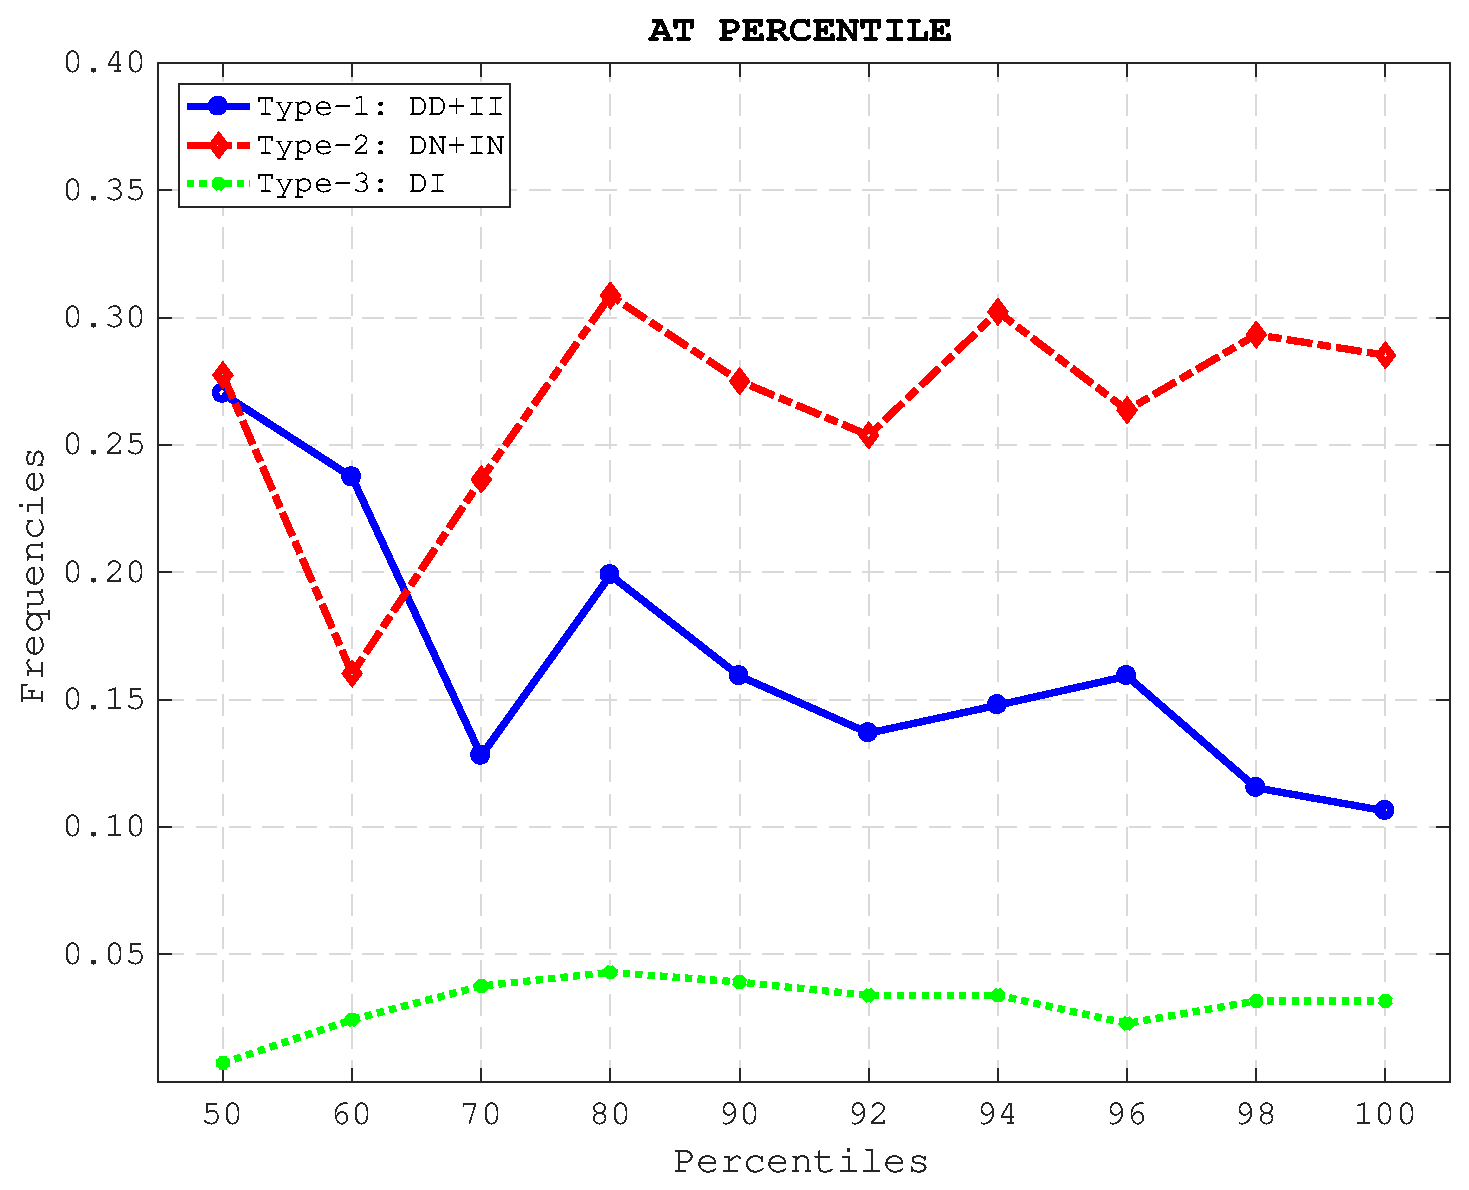
\includegraphics[width=4.25in]{pricecoordination_figure1}\\\medspace\\
	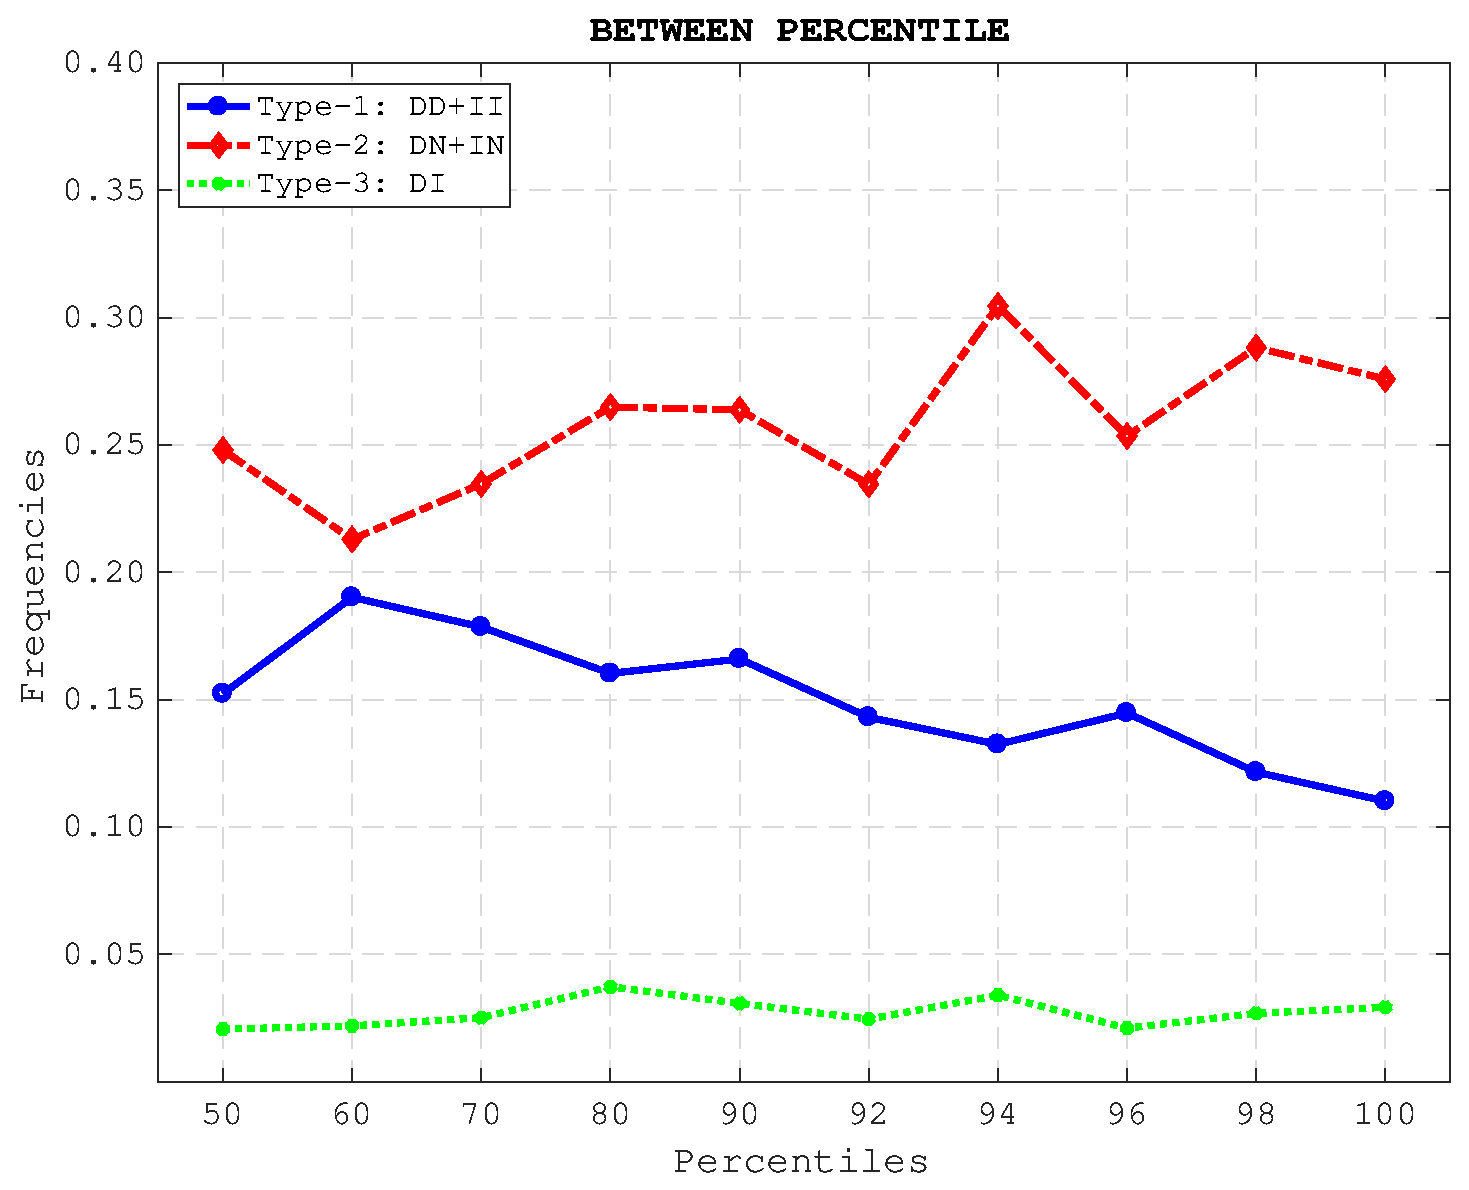
\includegraphics[width=4.25in]{pricecoordination_figure2}\\
	\caption{Price Coordination Within Name Groups Across Group Sizes: GP-D}
	\label{fig1}
\end{figure}

On the other hand, for GP-D, there is one conclusion can be reached, using the three-type definition of price coordination. See Fig \ref{fig1}.
\begin{itemize}
	\item As the size of the group increases, the price co-movement decreases (blue), while the price not-opposite-movement increases (red dashed), provided the price opposite-movement is about the same across percentiles (gree dotted).
	\item Such behavior is robust, in the sense that, this behavior is seen in both AT-percentile (upper panel) and in BETWEEN-percentile (lower panel).
\end{itemize}

\subsection{Price Coordination Within and Across Regions}

In this subsection, I report the price coordination within regions (EU \& NA \& NO), and across regions (EUNA \& EUNO), as well as price coordination without region classification (ALL).

As before, the main (puzzling) theme is that, price coordination within Euro-dollar region (EU) is about the same as that 
\begin{itemize}
	\item within regions that do not share currency, i.e., NA \& NO,
	\item across regions, i.e., EUNA \& EUNO, and
	\item within ``world'' region, i.e., without any region consideration (ALL).
\end{itemize}
This result strongly rejects the currency union being an underlying factor in price changes. In what follows, I report the frequency using PC-1 and GP-1, -3, -5, -9, and -13. See Table \ref{tbl4}.

\begin{table}[H]
	\caption{Price Coordination Price Coordination Within and Across Regions}\label{tbl4}
	\begin{tabular}{llrrrrrr}
		\hline\hline
		& Region & FRQ: DD & FRQ: II & FRQ: DN & FRQ: IN & FRQ: DI & FRQ: NN \\ \hline\hline
		GP-1  &        &         &         &         &         &         &         \\
		(1)   & EU     &   0.020 &   0.038 &   0.136 &   0.220 &   0.034 &   0.552 \\
		(2)   & NA     &   0.016 &   0.036 &   0.134 &   0.270 &   0.027 &   0.517 \\
		(3)   & NO     &   0.017 &   0.049 &   0.134 &   0.264 &   0.039 &   0.497 \\
		(4)   & EUNA   &   0.015 &   0.035 &   0.145 &   0.250 &   0.028 &   0.527 \\
		(5)   & EUNO   &   0.017 &   0.037 &   0.142 &   0.259 &   0.031 &   0.513 \\
		(6)   & ALL    &   0.018 &   0.040 &   0.139 &   0.255 &   0.034 &   0.514 \\ \hline
		GP-3  &        &         &         &         &         &         &         \\
		(1)   & EU     &   0.037 &   0.061 &   0.112 &   0.216 &   0.041 &   0.533 \\
		(2)   & NA     &   0.027 &   0.037 &   0.116 &   0.231 &   0.026 &   0.564 \\
		(3)   & NO     &   0.028 &   0.062 &   0.109 &   0.234 &   0.037 &   0.530 \\
		(4)   & EUNA   &   0.024 &   0.048 &   0.125 &   0.224 &   0.032 &   0.547 \\
		(5)   & EUNO   &   0.031 &   0.055 &   0.117 &   0.238 &   0.036 &   0.522 \\
		(6)   & ALL    &   0.031 &   0.058 &   0.114 &   0.233 &   0.037 &   0.526 \\ \hline
		GP-5  &        &         &         &         &         &         &         \\
		(1)   & EU     &   0.037 &   0.061 &   0.112 &   0.216 &   0.041 &   0.533 \\
		(2)   & NA     &   0.027 &   0.037 &   0.116 &   0.231 &   0.026 &   0.564 \\
		(3)   & NO     &   0.028 &   0.062 &   0.109 &   0.234 &   0.037 &   0.530 \\
		(4)   & EUNA   &   0.024 &   0.048 &   0.125 &   0.224 &   0.032 &   0.547 \\
		(5)   & EUNO   &   0.031 &   0.055 &   0.117 &   0.238 &   0.036 &   0.522 \\
		(6)   & ALL    &   0.031 &   0.058 &   0.114 &   0.233 &   0.037 &   0.526 \\ \hline
		GP-9  &        &         &         &         &         &         &         \\
		(1)   & EU     &   0.036 &   0.055 &   0.120 &   0.214 &   0.039 &   0.536 \\
		(2)   & NA     &   0.028 &   0.032 &   0.127 &   0.231 &   0.027 &   0.555 \\
		(3)   & NO     &   0.029 &   0.059 &   0.117 &   0.236 &   0.036 &   0.523 \\
		(4)   & EUNA   &   0.025 &   0.042 &   0.136 &   0.221 &   0.032 &   0.545 \\
		(5)   & EUNO   &   0.030 &   0.049 &   0.126 &   0.239 &   0.035 &   0.522 \\
		(6)   & ALL    &   0.031 &   0.052 &   0.122 &   0.234 &   0.036 &   0.525 \\ \hline
		GP-13 &        &         &         &         &         &         &         \\
		(1)   & EU     &   0.036 &   0.054 &   0.120 &   0.214 &   0.038 &   0.538 \\
		(2)   & NA     &   0.028 &   0.032 &   0.127 &   0.231 &   0.027 &   0.555 \\
		(3)   & NO     &   0.029 &   0.058 &   0.117 &   0.235 &   0.036 &   0.524 \\
		(4)   & EUNA   &   0.025 &   0.041 &   0.135 &   0.221 &   0.032 &   0.546 \\
		(5)   & EUNO   &   0.030 &   0.048 &   0.125 &   0.239 &   0.034 &   0.523 \\
		(6)   & ALL    &   0.030 &   0.052 &   0.122 &   0.234 &   0.036 &   0.526 \\ \hline\hline
	\end{tabular}
\end{table}
